% Intended LaTeX compiler: pdflatex

  \documentclass[a4,p11]{article}
  \usepackage[dvipdfmx]{graphicx}
  \usepackage[utf8]{inputenc}
  \usepackage[T1]{fontenc}
  
\usepackage[utf8]{inputenc}
\usepackage[T1]{fontenc}
\usepackage{graphicx}
\usepackage{grffile}
\usepackage{longtable}
\usepackage{wrapfig}
\usepackage{rotating}
\usepackage[normalem]{ulem}
\usepackage{amsmath}
\usepackage{textcomp}
\usepackage{amssymb}
\usepackage{capt-of}
\usepackage{hyperref}
\author{bob}
\date{}
\title{}
\hypersetup{
 pdfauthor={bob},
 pdftitle={},
 pdfkeywords={},
 pdfsubject={},
 pdfcreator={Emacs 26.1 (Org mode 9.1.9)}, 
 pdflang={Jp}}
\begin{document}


\section{abstract}
\label{sec:orgd2f022c}
At graduate research, 
although the process is more important than the results,
most students don't notice it.
Because the guild system is nice to learn the process,
the graduate reseach possesses a kind of
relationship between 
a mentor and a padawan learner.

On this project, 
we are developing a system for
noticing importance of learning process,
ornb, whose specifications and 
the connections to a static web system, jekyll,


\section{Introduction}
\label{sec:org3fafc48}
\subsection{ゼミナール}
\label{sec:orgd8b3bc5}
卒業研究などのゼミナール(以下、ゼミ)は,フンボルト理念を基礎としている.その通説を潮木は次のようにまとめている.
\begin{quote}
近代大学の出発点は1810年に創設されたベルリン大学である。この大学の基本構想を作ったのは、ヴィルヘルム・フォン・フンボルトであり、近代大学はこのフンボルト理念から始まった。フンボルト理念の中核は研究中心主義にある。つまり、大学は教育の場である以上に研究の場であるという考え方は、このフンボルトから始まった。これがドイツばかりでなく、世界の大学を変えた。- アルカディア学報(教育学術新聞掲載コラム),No.246
\end{quote}
と. また,「大学が伝えるべきことは,
いかにして新たな知識を発見するか,いかにして知識を進歩させるか,
そのための技法である」との観点から,「研究する学生」
を志向したとしている.

今日の学生が,このような深遠な思想を理解して,
長い受動的学習の最終段階として,ゼミに参加している気概は
感じられない.
また、最新の「教育」を行うと看板を掲げている大学に通う今日の学生は,
大学は研究の場であるという認識はなく,
卒業研究や,研究室におけるゼミへの参加に
どのようなスタンスで取り組むべきか迷っている.
研究のための予備知識,スキルの習得に役立つとして課されている
レポートや試験などは,
新しい発見につながる途中経過を求めているにもかかわらす,
既存の知識の暗記という結果のみを求めているという誤ったメッセージとして受け取られている可能性がある.
実践的な課題を,project based learning[Bell, 2010]や
active learning[Settles, 2009]として取り入れる試みがなされている[溝上慎一, 2007]が,
かける時間の割に,成果をあげるのが難しいとされている.

「研究する学生」を育てるには,個人に適合した指導が欠かせない.
これはある意味,メンターとメンティ,あるいは
マスターとパダワンのような関係となる.
しかし,ゼミナールへやってくる学生は,
研究指導が徒弟制的な制度であるとは全く予想していない.

\subsection{目的}
\label{sec:org280b74c}
次節で示す通り,このような旧態然とした徒弟制も現代的な視点で
見直しが進められている.
本プロジェクトで提供しようとするシステムは,
\begin{itemize}
\item 研究室は徒弟制
\item 学生はそれを知らない
\end{itemize}
という前提のもとで,徒弟制を現代的で新たな学習形態として提供することを
目的としている.

次節では,どのような経緯で徒弟制が見直されて来たか,また,
学習がAM/PMという視点によってどのように捉えられているかを
明らかにする.
その上で,近代的な徒弟制を研究室活動に導入するのに
必要となる仕様を列挙し,それに基づいた実装デザインを示す.

\section{徒弟制の見直し}
\label{sec:org3615d37}
\subsection{状況に埋め込まれた学習}
\label{sec:org55b4269}
1991年にレイヴとウェンガーによって,
  「状況に埋め込まれた学習」あるいは「正統的周辺参加」
  という学習形態・概念が提案された[福島真人, 1993].
  彼らは,アフリカの仕立て職人や助産婦の育成法を社会学的に詳しく調査した結果,
  徒弟制のなかに学びの本質があると指摘した.
少し複雑ではあるが,その概念をもっとも短くまとめたと思われる箇所を以下にそのまま書き写す.
\begin{quote}
学習はいわば参加という枠組で生じる過程であり,
個人の頭の中でではないのである.
このことは,とりもなおさず,
共同参加者の間での異なった見え方の違いによって学習が媒介されるということである.
この定義では「学ぶ」のは共同体である,
あるいは少なくとも,
学習の流れ(context)に参加している人たち,といえよう.
学習はいわば,共同参加者間にわかち持たれているのであり,
一人の人間の行為ではない.
生産過程では徒弟(見習い)が益々増大していく
参加によってきわめてドラマティックに変容していくものではあるが,
この変容の発生の場と発生の条件は,さらに広範囲の過程そのものである.
徒弟の親方たち自身が共同学習者としてふるまうことを通しどれほど変化するか,
したがって,習熟されている技能でもその過程でどれほど変化するか.
実践者の共同体がより大きくなると,
徒弟の形成によって共同体は自らを再生させるが,
同時に変容もすると考えられる.
LaveWenger[pp.8-9]

中略

また新参者を親方,ボス,あるいは管理者と深く対立する関係に陥らせる,参加させるよりも非自発的に隷従させるなど,これらの条件は実践における学習の可能性を部分的に,もしくは完全に,歪めてしまうと唱えた.
 LaveWenger[p.42]
\end{quote}
と記している.


\subsection{AM/PM}
\label{sec:org2f7fb33}
1998年数学者のSfardは,Lave and Wengerの考えを受け,
学習者,教授者,研究者の知識に対する心持ちを
AM(Acquisition Metaphor)とPM(Participation Metaphor)と名付けて分類した.
表\ref{tab:orgc5961f0}に示した通り,
学習に対する従来の考え方であるAMは,個人が知識を習得することを目標とし,
「学習」とは何かを獲得することであった.
また,「知る」とは個人が所有するものであるとしていた.
一方で学習に対する新しい考えであるPMは,学習の目標は共同体の構築であり,
「学習」とは参加者となることである.
本プロジェクトでは、学習者は,徒弟であり,教授者は,有識の参加者と定義した.
つまり,個人ではなく,教授者,学習者が共同体(チーム)として,
また徒弟制を築くことでお互いの知識構築がはかどる仕組みとなっている.

\begin{table}[bt]
\caption{\label{tab:orgc5961f0}
Acquisition metaphorとParticipation metaphorの比較.}
\centering
\begin{tabular}{lll}
\hline
Acquisition metaphor & 要素 & Participation metaphor\\
\hline
個人を豊かにする & 学習の目標 & 共同体の構築\\
何かを獲得する & 学習するとは & 参加者となる\\
受容者,再構築者 & 学習者 & 周辺参加者,徒弟\\
供給者,促進者,仲裁人 & 教授者 & 有識の参加者\\
資産,所有物,一般商品 & 知識,コンセプト & 実践,論考,活動の一側面\\
持つ,所有する & 知るとは & 所属する,参加する,コミュニケーションをとる\\
\hline
\end{tabular}
\end{table}

\subsection{PMの実践例と学生の受け止め方}
\label{sec:org3ba5fb7}
\subsubsection{ペア評価の意図}
\label{sec:org88a0800}
関西学院大学理工学部・情報科学科で
西谷が,PM,すなわち参加型学習の実践としての試みに,
数式処理演習という3年生向けの演習を実践している.
学生は好きなもの同士がペアを組み,
授業中課題や期末試験をペアで受け,
ペアの点数は全く同じとなる.
ペアで「相方の足を引っ張らないように」
という思考に至り,
互いが怠けることなく,
授業や課題に意欲的に取り組む.
その結果,互いに高め合い,知識の定着につながる.
この授業への取り組みの根底にあるのが、「共同体の構築」,「参加する」であり、
PMの実践を意図している.
しかし,実際には知識の定着に至らない学生が多数いる.
\subsubsection{学生の見え方}
\label{sec:orgc2b5f8e}
なぜ,
\begin{itemize}
\item 一つ目の要因はペアによる演習のため,
一人が作業すれば課題をクリアできる点である.
つまり,問題毎に役割を振り分け 
片方が問題を解いている時,
もう片方は携帯を見るなど考える事を
完全にやめることがある.
一緒に考えることをせず,
「休憩」の時間を作ることで
知識定着を目的とするのではなく,
課題達成,単位習得の事のみを考えた結果である.

\item 二つ目は,ペアで課題を一つ提出することが,
いわゆる出席点となるため
一人が授業を欠席しても,
点数が減点されることがない点である.
これは,一つ目に述べた要因より酷い例であり,
日にち毎に出席する担当を決めることで
授業に出席,参加すらしない場合があった.
\end{itemize}

結果的に学生的視点から見ると、
この授業はPMといった考え方を気づかせる授業ではなく
学生にとって,「授業に出なくても良い楽に単位を取れる授業」
という風に見受けられた.

個人での学習よりも互いに高め合い,
知識・スキルを習得するといったペアは一部であり,
優秀な学生と,そうでない学生がペアを組んだ場合,
前者がほとんどの課題をこなし,
後者はほとんど考えないというパターンも存在した.

これら一連のなぜを考えると、次の疑問が湧いてくる.
はたして、PMを理解して共同体を作ろうとまで考える学生はいたのだろうか?

教育の非対称性,
\begin{itemize}
\item 教える側はどう役にたつかを知っているが,
\item 教わる側は,知識を獲得するまでわからない.

\item サボりたい
\item 教わることはどこで役にたつかわからない
\item 役に立たない
\end{itemize}

ならば,単位取得で縛りましょう.
となるが,それでは伝統的な徒弟制となんら変わりはない.
どうすれば,役に立つことに学生が気づくのか.

\section{構築システムのアイデア}
\label{sec:org3de8c4e}
「新しい徒弟制」という視点に立って,研究室運用システムとして
\begin{itemize}
\item 日々の個人活動を構成員に公開する(blogシステム)
\item ペアによる個別指導(遠隔ペアプロ)
\item 欠席者のフォロー(スタンプ集め)
\end{itemize}
という機能提供することを当初の目標とした.

\subsection{blogシステム}
\label{sec:orgbd72b80}

\begin{figure}[htbp]
\centering
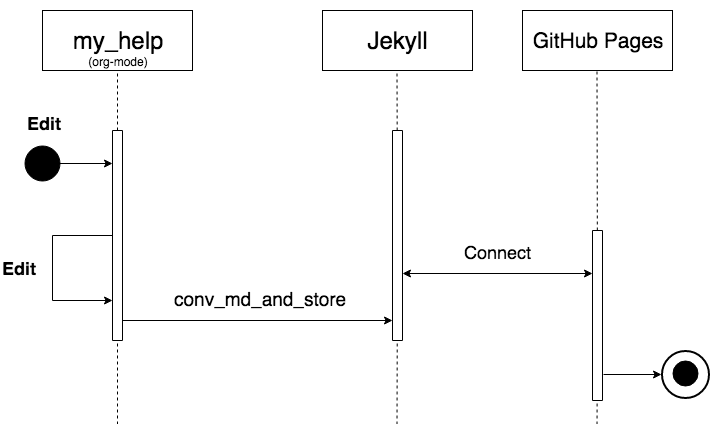
\includegraphics[width=.9\linewidth]{./images/myhelp_to_jekyll.png}
\caption{\label{fig:org97a2703}
blog作成から公開までの流れ.}
\end{figure}

学生個人のゼミ活動はゼミ発表などであるが,
より細かな活動を記録することが望ましい.
実験系の研究室では,研究室ノートや実験ノートなどで
日々の活動を記録する習慣をつけるが,
プログラミングを主体とする研究室においては
何行書いたを聞く指導教員もいる.
より良いプログラマの習慣は,
活動記録としてblogの公開が推奨されている.
これによって,
\begin{itemize}
\item どのようなアイデアで
\item どこで何を調べて
\item どこで挫折したか
\end{itemize}
などを公開することで,codingがうまくいかなかったとしても,
思考の過程を記録し,先輩や同僚のcode reviewを通じて,
programming skillの向上が期待される.
また会社においては,これは日報にも通じている.

研究室内の活動においても実践可能なblogシステムを目指して,
\begin{itemize}
\item my\_help
\item org-mode
\item jekyll
\end{itemize}
のそれぞれの機能を利用して実装した.
blogの作成から公開までの流れは図\ref{fig:org97a2703}のようになる.

\subsubsection{my\_help = 直交補空間}
\label{sec:org36e4e91}
my\_helpはRubygemsで提供されている,
ファイル構造において,メモやレポートが増えればchunkingの必要が出てくる.
ところが,chunkingすることにより,ディレクトリ構造が深くなる.
その結果,レポートやメモの場所が把握できなくなる.
これに対して,my\_helpは直交補空間を実現した知識構築を補助するツールである.
ディレクトリに拘束される事なく,
メモやレポートを作成・管理できるという利点があるため,
どこからでもアクセスできる.
my\_helpではBlogという形で文書を作成し,構成員に日報を伝える.

\subsubsection{org-mode = 便利なmark down}
\label{sec:org0d8d0c0}
org-modeは,Emacs上で動作するアウトライナーであり
プレーンテキストの文書作成環境である.
ノートの保存,TODOリストの管理,スケジュールや時間の管理,
また発表原稿やスライドの作成など様々な用途に対応している.
また,コードの実行はもちろん,リンク付け,テーブル表記の入力,
図や表の表示,ライブ計算,HTMLや\LaTeX{}への変換等の
機能も兼ね備えている.
今回のレポートとなる文書の作成するために,org-modeを用いる.

\subsubsection{jekyll = 晒すと何がいい?}
\label{sec:org412297a}
my\_helpはemacsのorg-modeを利用しているが,個人での使用を
前提としており,公開するためのシステムが存在しない.
jekyllはRubygemsで提供されている静的サイトジェネレーターである.
テーマや構成を変更することができ,好みのサイトを作成できる.
Githubには,Jekyllで作成されたサイトを公開する
GitHub Pagesというサービスが用意されている.

my\_helpで作成されたBlogを,Jekyllに連携することで,
localにおいてその完成度を確認することができる.
また,git pushするだけでgithub pagesでworld wideに公開される.


\subsection{遠隔ペアプロ}
\label{sec:orged89ac6}
ペアの活動や欠席者の遅れをフォローするシステムを提供する.
現在,ゼミを中心とした,個別の時間調整を行っている.
しかし,1週間学校に来れない人もいるため,
それを援助すべく遠隔でもペアプロや知識の共有をする.

ペアプロが機能する理由は,
\begin{quote}
ただ始めること.これがたぶん生産性の鍵なのだ.
ペアプロが機能する理由は,「相方とペアプロ作業を予定する」ことで,
「作業を始めることをお互いが強制する」からに違いない
(原文より訳出).
Joel Spolsky 著,青木靖訳「Joel on software」(オーム社,2005)p.133.
\end{quote}
であるとされており,空間を共有する必要はない.

キャンパスが郊外にあるため,効率的にゼミナールの研究を進めるためには,
遠隔での共同作業が不可欠である.そこで,いくつかの環境を使って
実際の作業を試行して,結果を収集する.

そのような環境で必要となる仕様は,新しいタイプの徒弟制の視点に立って,
\begin{enumerate}
\item 先輩と後輩によるペアプロ
\item コードのリアルタイム共有
\item 音声,ポインタなどによる指示
\item 作業記録,振り返り
\end{enumerate}
などが効率的に行えることである.

\subsection{スタンプ集め}
\label{sec:orgd581cf7}

また,構成員は教授者と学習者の両方に成り得るものとし,欠席者は
ゼミ出席者を教授者としゼミの内容や課題を教えてもらう学習者とする.

学習者は,教授者に教えてもらいながら,
課題に取り組むとともに,Blogを作成し,知識定着をはかる.
課題達成後は教授者が学習者にスタンプを押す.
そのスタンプが,課題達成の証明となり,卒業するまでの必須
過程とする.
また,ゼミ欠席者でも教授者にスタンプを押してもらうと,
教授者としての資格を獲得し,
他の欠席者に教える事ができ,課題達成後はスタンプを押す.

ゼミ毎にスタンプを用意し,全てのスタンプの取得が卒業の必須項目とする.

例えば
\begin{itemize}
\item 全員jekyllを入れて,blogを晒す
\end{itemize}
というゼミで実行した課題があるとする.
そいつを全員が実行したかどうかを,教えた方がチェックする.

手順は以下の通り,
\begin{itemize}
\item 欠席者が出席者に聞く
\item 出席者がスタンプを押す
\item それが埋まってなかったら卒業なし.
\end{itemize}
これを自動化するシステム.

いっぺん聞いたら他の人に教えるのはあり.
そうすると,教えることによる記憶強化の可能性が高まる.
また,不明瞭な点のあぶり出しが可能になる.

\section{今後の課題}
\label{sec:org9966a70}

\section{引用文献}
\label{sec:org2b1d460}
\begin{itemize}
\item\relax [潮木] フンボルト理念,神話の崩壊
\item\relax [溝上慎一, 2007]
溝上慎一, アクティブ・ラーニング導入の実践的課題, 名古屋高等教育研究,第7号,pp.269--287(2007)
\item\relax [Bell, 2010]
S. Bell, ‘Project-Based Learning for the 21st Century: Skills for the Future’, The Clearing House: A Journal of Educational Strategies, Issues and Ideas, vol. 83, no. 2, pp. 39–43, Jan. 2010.
\item\relax [Settles, 2009]
B. Settles, ‘Active Learning Literature Survey’, University of Wisconsin-Madison Department of Computer Sciences, Technical Report, 2009.
\end{itemize}
\end{document}
